\section{Transport and installation}



\subsection{Life cycle}

Find everything you need to know after you ordered your HT500.3 3D Printer in the following paragraphs. From the day of your invoice until the day you want to dispose of the apparatus and anything in between is explained here. 


\subsubsection{Delivery}

The HT500.3 3D Printer arrives at your place fully assembled and can be commissioned directly after setting it up and connecting the power supply.
The 3D Printer is delivered in a transport box on a palette. It is advisable to leave the HT500.3 packed and on the palette until moving it to its final installation site for commissioning.
At the installation site, unpack the HT500.3 according to the information in the accompanying Quick Start Guide.
Dispose of the packaging in accordance with the local waste disposal regulations.
After unpacking, inspect the apparatus for:

\begin{itemize}
  \item damage in transit
  \item completeness of the delivery (compare delivery note)
\end{itemize}

If you notice any deviants, please immediately inform the hauler and the manufacturer. \emph{Do not} put the HT500.3 to use with defective parts.


\subsubsection{Transport}

To avoid injuries and property damage observe the following notes when transporting the HT500.3:

\begin{itemize}
  \item The apparatus' weight exceeds 50 kg. Always carry it \emph{two by two}.
  \item Keep the HT500.3 horizontal to avoid damaging internal parts.
  \item Avert shock loads to the housing.
\end{itemize}


The HT500.3 has been designed for stationary application. It is not equipped with special transport devices such as lifting eyes or handles. The feet provide sufficient clearance to lift the apparatus and carry it to the installation site.
While the HT500.3 is packed and on its transport palette, use a lifting cart or pallet stacker for transportation. Make sure that the weight is evenly distributed and secure the HT500.3 against tilting. 

\begin{info}
  The housing is not designed for subsequently attaching lifting eyes. If you need to transport the 3D Printer longer ways, load and secure it on a stable pallet and transport it with a pallet stacker or lifting cart.
  Detailed information about safeguarding and packing the 3D Printer for shipping can be found in the Service Guide.
\end{info}


\subsubsection{Storage}

If the HT500.3 must be stored away, choose a leveled storage site and make sure that the 3D Printer does not stand on a ledge.
Before storing it, clean the HT500.3 and protect it from dust with a plastic tarpaulin or air cushion foil.

\begin{notice}
  Do not cover the 3D Printer with a textile sheet since the fibers may enter the supply system and clog the nozzles after recommissioning. Use lint-free plastic sheets only.
\end{notice}

The storage ambient conditions for the HT500.3 and its components are stated in the data sheet. For recommissioning after lengthy periods of storage follow the information given in initial commissioning. 


\subsubsection{Environment, recycling and disposal}

When used as intended, the HT500.3 presents no environmental danger.
However, the internal cooling works with a coolant that can be environmentally dangerous when leaking (see data sheet). Please observe the manufacturer's safety data sheet when handling the coolant.
The materials used for printing can also be environmentally dangerous when handled improperly. Always observe the manufacturer's safety data sheet and process plastics only within the limit values specified therein and with respect to the safety instructions.

\emph{Generally, consider the environment}: the auxiliary and operating materials of the HT500.3 can be dangerous to environment and health.
Awareness and foresighted behavior help avoiding ecological and personnel damage.
Components may bear valuable elements such as rare earths, or may be reusable. Do not waste them by inadequate and thoughtless disposal.
Environmentally hazardous substances \emph{must not} trickle into the soil or enter the sanitation. They must be stored in suitable containers and be disposed off adequately and in accordance with local and national regulations.

The HT500.3 is recyclable due to its low-pollution equipment. Nonetheless, the European Guideline 2002/96/EG (Waste Electrical and Electronic Equipment - WEEE) and the German \emph{Elektro- und Elektronikgesetz} (ElektroG) forbid the disposal of the apparatus via the household garbage. For environmental friendly recycling and disposal of the HT500.3 please contact a certified electronic waste management professional.

\begin{info}
  Kühling\&Kühling emphasize that there is no redemption obligation in this regard.
\end{info}



\subsection{Setup and Installation}

Use a lifting carriage to bring the HT500.3 on its transport pallet as near to its setup site as possible. Before setting up the HT500.3 remove the lid and side walls of the transport box and all straps. Subsequently, lift the apparatus off the transport pallet two-by-two and carefully carry it to its final installation location. 

\subsubsection{Installation requirements}

\begin{notice}
  The apparatus must not be set up in a surrounding with high formation of dust (e.g. near woodworks etc.). Ingress of particles into the filament supply system can lead to intense cleaning efforts due to clogging of the nozzles and thus immense non-productive time.
\end{notice}

Set up the HT500.3 at a well aerated place with an all-season ambient temperature between 15 and 25\degree C and a maximum relative humidity of 70\%.
Position the HT500.3 on a flat, carrying and enduring surface with a load capacity of at least 75 kg.
To ensure unhindered aeration of the electronic chamber no soft, movable materials (e.g. table cloth, cardboard strips, paper etc.) may be placed underneath the apparatus to prevent clogging of the vent slots.
The required setup space must at least be 650 x 650mm and provide approximately 500mm free space to either side to enable unhindered access to the electronic chamber for service and maintenance work. At least 750mm free space must be left at the back of the HT500.3 to make changing the material easy and to ensure free air circulation at the ventilation grill in the back cover. At the front a free space of 1.250mm is recommended to allow easy operation with open chamber doors.
To easily access the touchscreen in a sitting or standing position the height of the setup table should not undercut 780mm.
A 230V power source must be within the range of the connection cable. 


\subsubsection{Unpacking the machine}

\begin{figure}[H]
  \centering
  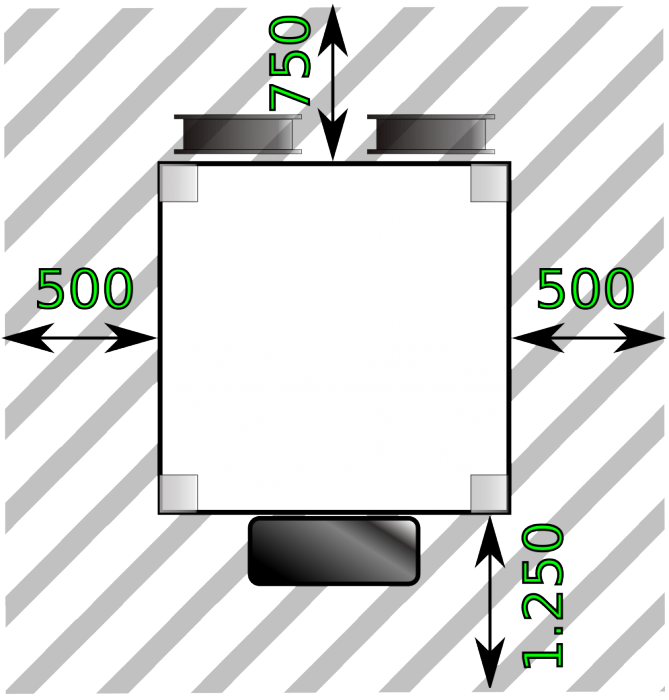
\includegraphics[width=.7\linewidth]{./img/workspace.png}
  \caption{Necessary free space around the HT500.3}
\end{figure}

\begin{danger}
  OF CUTTING INJURIES AND EYE DAMAGE\\
  The packing straps are pretensioned and may whip when cut, causing cutting injuries or eye damage.
  \begin{itemize}
    \item Hold down the top part of the strap and cut it at the side. Make sure it does not hit somebodies face.
  \end{itemize}
\end{danger}

\begin{danger}
  OF CUTTING INJURIES\\
  The transport box is made of unfinished plywood and may hold splinters and sharp edges that can cause cutting injuries.
  \begin{itemize}
    \item Take care when removing the transport packaging and wear protective gloves.
  \end{itemize}
\end{danger}

\begin{notice}
  If the 3D Printer has a temperature below 16\degree C (e.g. directly after delivery in cold weather) there is a danger of air humidity condensing on sensitive electronic components. This can lead to severe damages due to short circuiting during commissioning.
  Therefore, it is necessary to thoroughly let the 3D Printer warm up to ambient temperature for at least 12 hrs. at its operating place 
  \emph{prior} to commissioning.
  Regard the ambient conditions required for operation.  
\end{notice}

To unpack the machine, cut the tensioning straps of the transport box, remove the lid and carefully lift the box over the printer.
Then cut the tensioning straps around the 3D Printer and remove the wooden cover plate and the air cushion foil.
Set aside and store all parts of the transport packaging for later use, e.g. moving or shipping the 3D Printer. 

\begin{figure}[H]
  \centering
  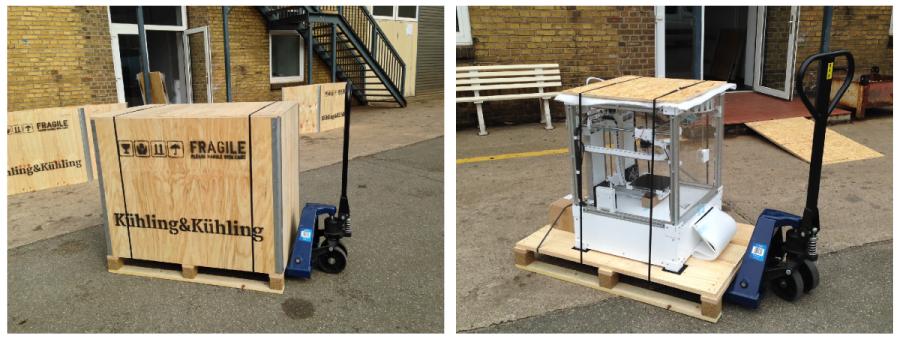
\includegraphics[width=.7\linewidth]{./img/secure_boxed.png}
  \caption{The box and the lid are fastened to the pallet with tensioning straps.
           The 3D Printer is padded with air cushion foil and a wooden cover plate and strapped to the pallet with tensioning straps.}
\end{figure}

\begin{info}
  Find detailed information on repacking the machine for shipping in the Service Guide.
\end{info}


\subsubsection{Removing the transport restraints}

All moving components of the HT500.3 3D Printer are secured with blue tape against damage in transit.
Make sure all transport restraints named in the adjacent pictures have been removed before commissioning the 3D Printer.

\begin{figure}[H]
  \centering
  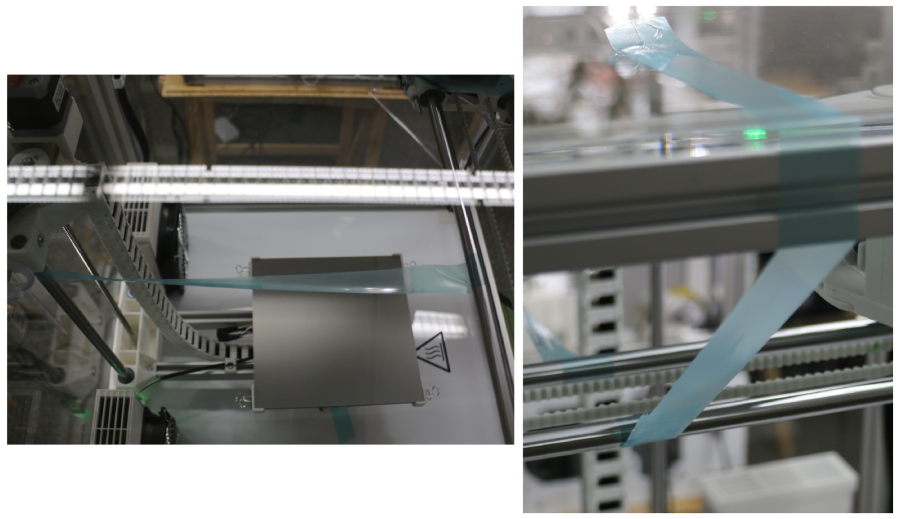
\includegraphics[width=.7\linewidth]{./img/secure_yaxis.png}
  \caption{Transport restraint of the Y-axis: blue tape spans from the hind Y-shaft to the left Z-shaft and from the front Y-shaft to the top 
           cover.}
\end{figure}

\begin{figure}[H]
  \centering
  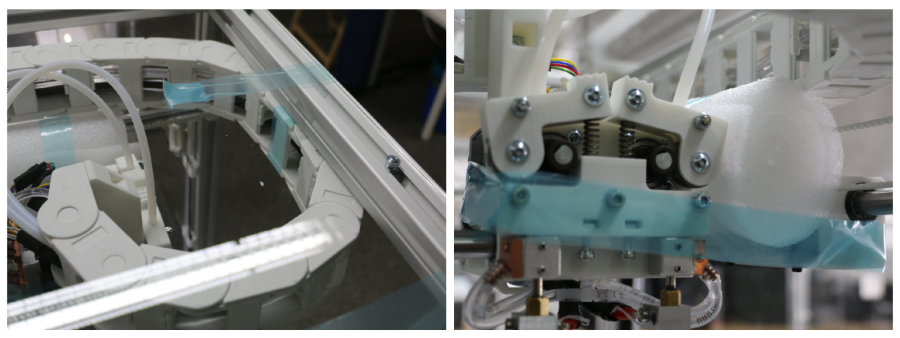
\includegraphics[width=.7\linewidth]{./img/secure_headchain.png}
  \caption{Transport restraint of the main e-chain: blue tape is strapped around the chain an fastened to the top cover.
           Transport restraint of the extruder head: the extruder head is cushioned with air cushion foil and strapped to the 
           right X-end with blue tape.}
\end{figure}

\begin{figure}[H]
  \centering
  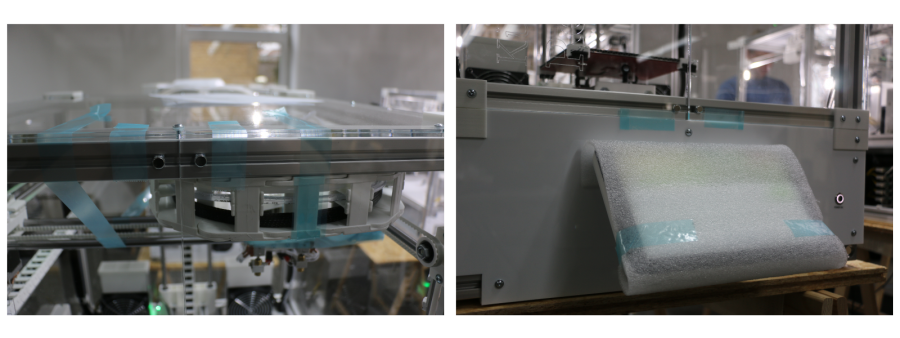
\includegraphics[width=.7\linewidth]{./img/secure_doors.png}
  \caption{The doors are held close by blue tape at the top and lower edge.
           The touchscreen is packed in air cushion foil.}
\end{figure}

\begin{figure}[H]
  \centering
  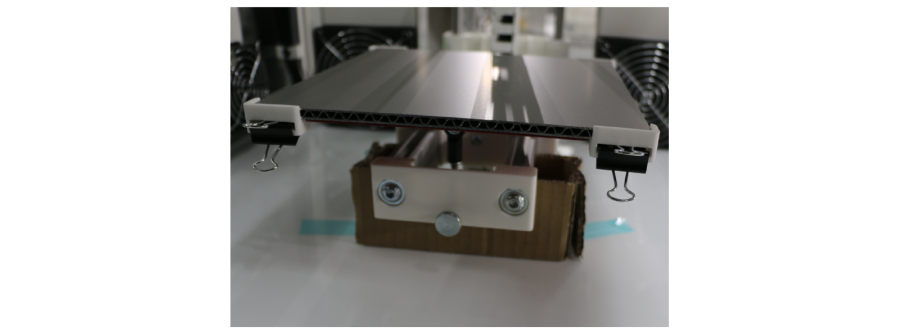
\includegraphics[width=.7\linewidth]{./img/secure_table.png}
  \caption{A cardboard frame supports the print table.}
\end{figure}


\subsubsection{Connections}

After setting the apparatus up it must be connected to the power supply and the data network.

\begin{enumerate}
  \item Set the power supply main switch at the back of the 3D Printer to \emph{<0>} (OFF).
  \item Unpack the supply cable and connect it to the mains plug at the backside.
  \item Connect the Schuko plug to a 230 V socket.
  \item Connect the HT500.3 to your data network by plugging the network cable into the RJ45 ethernet plug. 
        Your network must provide DHCP IP address management and should be connected to the internet (to enable the printer to fetch current time signal via Network Time Protocol (ntp)).
\end{enumerate}

\subsubsection{Initial commissioning}

After set-up has been completed the further commissioning of the HT500.3 takes place at the web interface and the touchscreen as described in the Operating Manual. 

\subsection{Decommissioning}

Decommissioning may be necessary on two occasions: the temporary decommissioning if the 3D Printer will just be out of operation for a limited time (e.g. moving) or the permanent decommissioning if the 3D Printer has expired its lifetime and will be scrapped.


\subsubsection{Temporary decommissioning}

 If you need to take the HT500.3 out of operation to move or store it, regard the following information:
\begin{itemize}
  \item Remove remaining filament from the supply system.
  \item Clean the 3D Printer, especially the extruder nozzles.
  \item Move all axes into their home positions.
  \item Disconnect the mains cable and the network cable. Store them together with the 3D Printer 
        (e.g. fixed with adhesive tape inside the build chamber).
  \item Protect the print table surface and the touchscreen with a cardboard pad against scratching.
  \item Secure the extruder head, the print table, and the build chamber doors with strapping tape tape against moving (see Transport).
  \item Position the 3D Printer on a transport pallet and cover it with a plastic tarpaulin or air cushion foil.
\end{itemize}

\begin{notice}
  Do not cover the 3D Printer with a textile sheet since the fibers may enter the supply system and clog the nozzles after recommissioning. Use lint-free plastic sheets only.
\end{notice}

\begin{itemize}
  \item Use lashing straps to secure the 3D Printer on the transport pallet. 
\end{itemize}


\subsubsection{Permanent decommissioning}

 If you do not want to use the HT500.3 any longer or if it is damaged beyond repair:
\begin{itemize}
  \item Take the HT500.3 out of operation as described above.
  \item Drain the cooling system and collect the coolant. 
        Dispose of the coolant according to your local guidelines and the manufacturer's data sheet.
  \item Disassemble all components according to their recyclablility and dispose of them adequately and lawfully.
\end{itemize}

\begin{info}
  Components may bear valuable elements such as rare earths, or may be reusable. Do not waste them by inadequate and thoughtless disposal.
\end{info}



\subsection{On demand maintenance}

The HT500.3 3D Printer features a low-maintenance design, thus intensive maintenance time is not required during normal operation. Nonetheless regard the maintenance intervals stated in the Service Guide.

Apart from this, regular cleaning will mostly suffice to keep your 3D Printer running satisfactorily.

